\chapter{Finite impulse response Theory} \label{app:FIR_theory}
This appendix will describe the theory of the FIR filter design method, which includes the Kaiser window method and calculating the b coefficients.

The requirements for a lowpass filter should be stated as on \autoref{fig:filter_req}.
\begin{figure}[H]
\centering
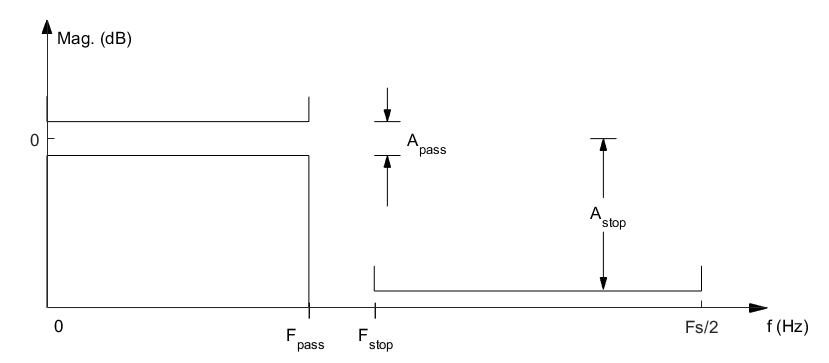
\includegraphics[width=0.8\textwidth]{figures/filter_req.png}
\caption{Requiremetns of a the lowpass filter.}
\label{fig:filter_req}
\end{figure}
From these the following conversion are made:
\begin{equation}
\omega_p=2\pi F_{pass}/Fs,\\
\omega_s=2\pi F_{stop}/Fs,\\
\delta_p=10^{A_{pass}/20},\\
\delta_s=10^{A_{stop}/20}
\end{equation}

The method used for deriving the order of the FIR filter will be the Kaiser window an is explained below.

\section{Kaiser window method}
The kaiser window method calculates the order of the filter and the beta value of the Kaiser window which is will be used to calculating the coefficients of the filter.

First the specification of the filter must be established: $\omega_p$, $\omega_s$, $\delta_p$ and $\delta_s$. For the kaiser window method the peak error $\delta$ will be the same in both the passband and stopband. which means: $\delta_p = \delta_s$ and the $\delta$ used is the lowest.

With the specifications established the cutoff frequency of the filter is found:
\begin{equation}
\omega_c=\frac{\omega_p+\omega_s}{2}
\end{equation}
Next the parameters for the Kaiser window must be determined:
\begin{equation}
\triangle\omega = \omega_s-\omega_p, \qquad\qquad A=-20log_{10}(\delta)
\end{equation}
The $\beta$ can the be calculated from:
\begin{equation} \label{eq:beta}
\beta=\left\{
\begin{array}{c l}      
    0,1102(A-8,7), & A>50,\\
    0,5842(A-21)^{0,4}+0,07886(A-21), & 21\leq A\leq 50\\
    0,0, & A<21.
\end{array}\right.
\end{equation}
and the order M can be calculated from:
\begin{equation}
M=\frac{A-8}{2,285\triangle\omega}
\end{equation}
Where M is predicted within $\pm$2. This leads to the calculation of the Kaiser window which is defined as:
\begin{equation} \label{eq:kaiserwindow}
w[n]=\left\{
\begin{array}{c l}      
    \frac{I_0[\beta(1-[n-\alpha)/\alpha]^2)^{1/2}]}{I_0(\beta)} & 0\leq n\leq M,\\
    0, & \textrm{otherwise},
\end{array}\right.
\end{equation}
Where $I_0$ is the zeroth-order modified Bessel function. The order of the FIR filter and the coefficients of the kaiser window can now be calculated and applied to the coefficients of the FIR filter which are derived below.

\section{Calculation of coefficients}
The calculation of the coefficients is done using the ideal frequency response as seen on \autoref{fig:IdealFilterApp}.
\begin{figure}[H]
\centering
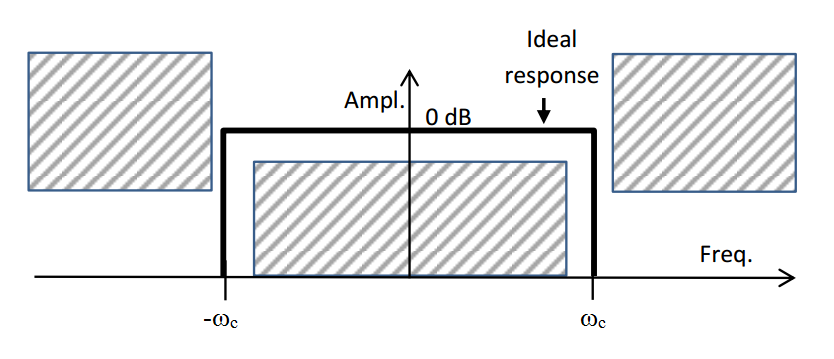
\includegraphics[width=0.6\textwidth]{figures/Ideal_filter.png}
\caption{The ideal frequency response of a lowpass filter.}
\label{fig:IdealFilterApp}
\end{figure}
Which is defined as:
\begin{equation} \label{eq:idealfreq}
H_d(e^{j\omega})=\left\{
\begin{array}{c l}      
    e^{\frac{j\omega M}{2}} & |\omega|\leq\omega_c\\
    0 & \omega_c\leq\pi
\end{array}\right.
\end{equation}
The ideal impulse response can be found taking the inverse Fourier transformation of \autoref{eq:idealfreq}
\begin{equation}
h_d[n]=\frac{1}{2\pi}\int_{-\omega_c}^{\omega_c}e^{\frac{j\omega M}{2}} e^{j\omega n} d\omega
\end{equation}
The two exponentials are subtracted to a single exponential:
\begin{equation}
h_d[n]=\frac{1}{2\pi}\int_{-\omega_c}^{\omega_c}e^{j(n-\frac{M}{2})\omega} d\omega
\end{equation}
Using Eulers rule:
\begin{equation}
h_d[n]=\frac{1}{2\pi}\int_{-\omega_c}^{\omega_c}cos\Big((n-\frac{M}{2})\omega\Big)+jsin\Big((n-\frac{M}{2})\omega\Big) d\omega
\end{equation}
\textbf{Forklaring} (Sin is an odd function)
\begin{equation}
h_d[n]=\frac{1}{2\pi(n-\frac{M}{2})}\bigg[sin\Big((n-\frac{M}{2})\omega\Big)\bigg]_{-\omega_{c}}^{\omega_{c}}
\end{equation}
where:
\begin{equation}
\int_{a}^{b}cos(ax) dx = \Big[\frac{sin(ax)}{a}\Big]_{a}^{b}
\end{equation}
The integral is expanded:
\begin{equation}
h_d[n]=\frac{1}{2\pi(n-\frac{M}{2})}\bigg[sin\Big(\omega_c(n-\frac{M}{2})\Big)-sin\Big(-\omega_c(n-\frac{M}{2})\Big)\bigg]
\end{equation}
where:
\begin{equation}
sin(-x) = -sin(x)
\end{equation}
Which means that the numenator is doubled equaling:
\begin{equation}
h_d[n]=\frac{sin\Big(\omega_c(n-\frac{M}{2})\Big)}{\pi(n-\frac{M}{2})}\qquad-\infty<n<\infty
\end{equation}
The impulse response is now symmetric around M/2 and the phase is therefore linear. The impulse response is still infinite and non-causal so the impulse response must be truncated.

The impulse response is truncated using the Kaiser window:
\begin{equation}
h[n]=h_d[n]\cdot w[n]\qquad\textrm{ where } w[n]\neq0 \textrm{ for } 0<n<M
\end{equation}
Which gives the coefficients of the designed lowpass type 1 FIR filter. 








